\section{SGLang Framework}
{{\footnotesize
\begin{description}[labelwidth=5em, labelsep=1em, leftmargin=*, align=left, itemsep=0.3em, parsep=0em]
  \item[date:] 2023-12-12
  \item[version:] TODO
  \item[last\_updated:] 2025-06
  \item[expired:] unknown
  \item[valid:] yes
  \item[valid\_date:] TODO
  \item[url:] \href{https://github.com/sgl-project/sglang/tree/main/benchmark}{https://github.com/sgl-project/sglang/tree/main/benchmark}
  \item[doi:] TODO
  \item[domain:] LLM Vision
  \item[focus:] Fast serving framework for LLMs and vision-language models
  \item[keywords:]
    - LLM serving
    - vision-language
    - RadixAttention
    - performance
    - JSON decoding
  \item[summary:] A high-performance open-source serving framework combining efficient backend runtime (RadixAttention, batching, quantization) and expressive frontend language, boosting LLM/VLM inference throughput up to \textasciitilde{}3x over alternatives. :contentReference[oaicite:5]\{index=5\}

  \item[licensing:] TODO
  \item[task\_types:]
    - Model serving framework
  \item[ai\_capability\_measured:]
    - Serving throughput
    - JSON/task-specific latency
  \item[metrics:]
    - Tokens/sec
    - Time-to-first-token
    - Throughput gain vs baseline
  \item[models:]
    - LLaVA
    - DeepSeek
    - Llama
  \item[ml\_motif:]
    - LLM Vision
  \item[type:] Framework
  \item[ml\_task:]
    - Model serving
  \item[solutions:] TODO
  \item[notes:] Deployed in production (xAI, NVIDIA, Google Cloud); v0.4.8 release June 2025. :contentReference[oaicite:6]\{index=6\}

  \item[contact.name:] SGLang Team
  \item[contact.email:] unknown
  \item[datasets.links.name:] Benchmark configs
  \item[results.links.name:] ChatGPT LLM
  \item[fair.reproducible:] Yes
  \item[fair.benchmark\_ready:] Yes
  \item[ratings.software.rating:] 0
  \item[ratings.software.reason:] Not analyzed.

  \item[ratings.specification.rating:] 8.0
  \item[ratings.specification.reason:] Clearly framed around surrogate learning across 16 domains, but not all tasks are formally posed or constrained in a unified benchmark protocol. Paper mentions performance on NVIDIA H100.

  \item[ratings.dataset.rating:] 9.0
  \item[ratings.dataset.reason:] FAIR-compliant physics simulation dataset, structured in HDF5 with unified metadata.

  \item[ratings.metrics.rating:] 7.0
  \item[ratings.metrics.reason:] Metrics like dataset size and domain coverage are listed, but standardized quantitative model evaluation metrics (e.g., RMSE, MAE) are not enforced.

  \item[ratings.reference\_solution.rating:] 9.0
  \item[ratings.reference\_solution.reason:] FNO and U-Net baselines available; full benchmarking implementations pending NeurIPS paper code release.

  \item[ratings.documentation.rating:] 10.0
  \item[ratings.documentation.reason:] Site and GitHub offer a unified API, metadata standards, and dataset loading tools; NeurIPS paper adds detailed design context.

  \item[id:] sglang\_framework
  \item[Citations:] \cite{zheng2024sglangefficientexecutionstructured}
  \item[Ratings:]
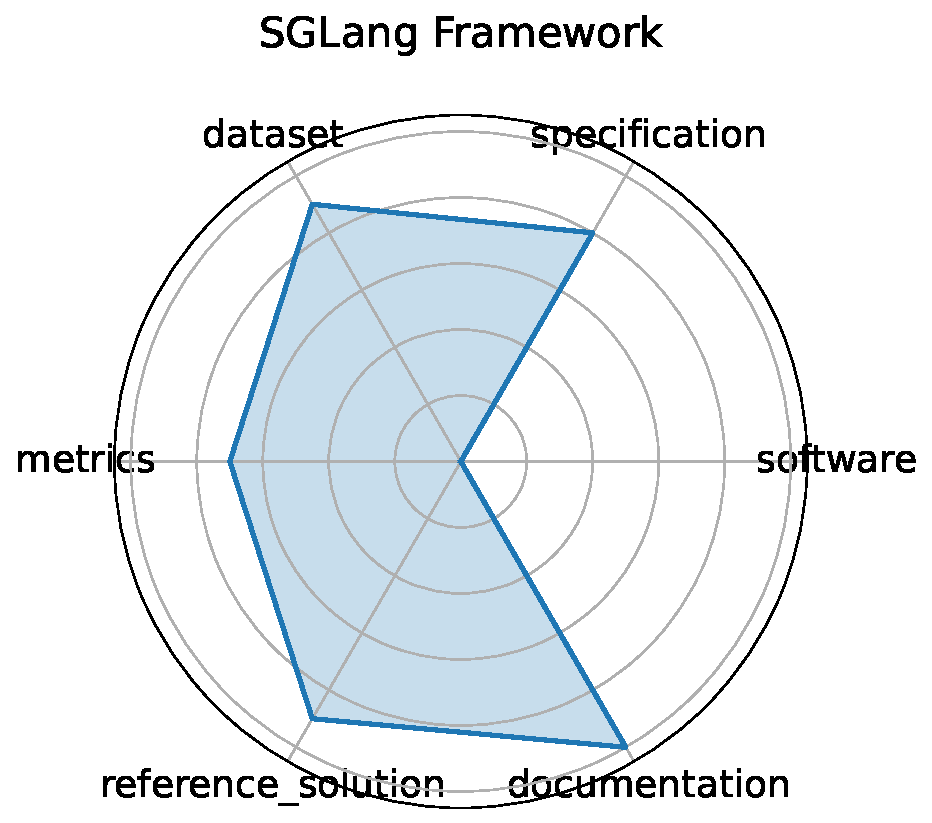
\includegraphics[width=0.2\textwidth]{sglang_framework_radar.pdf}
\end{description}
}}
\clearpage